\documentclass[a4paper,10pt]{article}
\usepackage{hyperref}

% For code example
\usepackage{listings}
\usepackage{xcolor}
\definecolor{codegreen}{rgb}{0,0.6,0}
\definecolor{codegray}{rgb}{0.5,0.5,0.5}
\definecolor{codepurple}{rgb}{0.58,0,0.82}
\definecolor{backcolour}{rgb}{0.95,0.95,0.92}
\lstdefinestyle{mystyle}{
    backgroundcolor=\color{backcolour},   
    commentstyle=\color{codegreen},
    keywordstyle=\color{magenta},
    numberstyle=\tiny\color{codegray},
    stringstyle=\color{codepurple},
    basicstyle=\ttfamily\footnotesize,
    breakatwhitespace=false,         
    breaklines=true,                 
    captionpos=b,                    
    keepspaces=true,                 
    numbers=left,                    
    numbersep=5pt,                  
    showspaces=false,                
    showstringspaces=false,
    showtabs=false,                  
    tabsize=2
}

\lstset{style=mystyle}

\usepackage{graphicx} % Required for inserting images
\usepackage[english]{babel}
%4 stackanchor  
\usepackage{stackengine}
% define nice looking boxes
\usepackage[many]{tcolorbox}

% a base set, that is then customised
\tcbset {
  base/.style={
    boxrule=0mm,
    leftrule=1mm,
    left=1.75mm,
    arc=0mm, 
    fonttitle=\bfseries, 
    colbacktitle=black!10!white, 
    coltitle=black, 
    toptitle=0.75mm, 
    bottomtitle=0.25mm,
    title={#1}
  }
}
\definecolor{brandblue}{rgb}{0.34, 0.7, 1}
\newtcolorbox{mainbox}[1]{
  colframe=brandblue, 
  base={#1}
}

\definecolor{orange}{rgb}{1, 0.55, 0.3}
\newtcolorbox{tbox}[1]{
  colframe=orange, 
  base={#1}
}

\definecolor{green}{rgb}{0.294, 0.729, 0.254}
\newtcolorbox{bembox}[1]{
  colframe=green, 
  base={#1}
}

\definecolor{red}{rgb}{0.99, 0.04, 0.99}
\newtcolorbox{tipbox}[1]{
  colframe=red, 
  base={#1}
}

\newtcolorbox{defbox}[1]{
  colframe=black!20!white,
  base={#1}
}
% Mathematical typesetting & symbols
\usepackage{amsthm, mathtools, amssymb} 
\usepackage{marvosym, wasysym}


\allowdisplaybreaks

% Tables
\usepackage{tabularx, multirow}
\usepackage{booktabs}
\renewcommand*{\arraystretch}{2}

% Make enumerations more compact
\usepackage{enumitem}
\setitemize{itemsep=0.5pt}
\setenumerate{itemsep=0.75pt}

% To include sketches & PDFs
\usepackage{graphicx}

% For hyperlinks
\usepackage{hyperref}
\hypersetup{
  colorlinks=true
}
% Math helper stuff
\def\limn{\lim_{n\to \infty}}
\def\limxo{\lim_{x\to 0}}
\def\limxi{\lim_{x\to\infty}}
\def\limxn{\lim_{x\to-\infty}}
\def\sumk{\sum_{k=1}^\infty}
\def\sumn{\sum_{n=0}^\infty}
\def\R{\mathbb{R}}
\def\dx{\text{ d}x}
\usepackage[utf8]{inputenc}

\title{Network Analysis Lecture Notes}
\author{Konstantin Lucny}
\date{HS 2023}

\begin{document}
\maketitle
\section{Lecture}
\subsection{Ties}
\begin{itemize}
    \item \textbf{Weak ties}: usually connected two different groups
    \item \textbf{strong ties}: usually connected people within one group
\end{itemize}
\begin{tipbox}
    {Weak becoming Strong ties}
    If two different groups would be connected through a strong tie, it is very likely that the two groups become one group. (Forbidden triad [see below] is hence very unlikely)
\end{tipbox}
\begin{figure}[h]
    \centering
    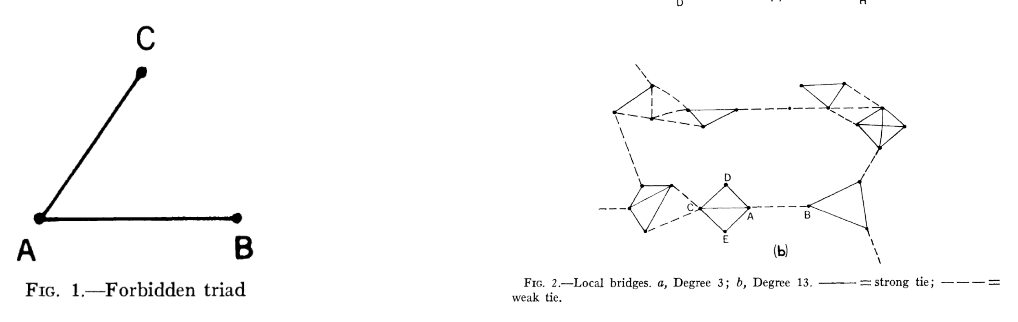
\includegraphics[width=1\linewidth]{Images/Example Networks.png}
    \caption{Example Networks; forbidden triad}
    \label{fig:enter-label}
\end{figure}
\pagebreak
\subsection{Describing a relation}
\begin{figure}[h]
    \centering
    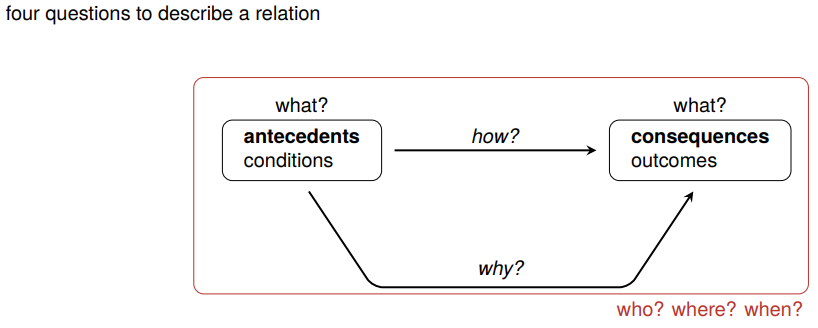
\includegraphics[width=1\linewidth]{Images/e2.png}
    \caption{Describing a relation}
    \label{fig:enter-label}
\end{figure}
\subsection{Theory \& Hypothesis}
\begin{itemize}
    \item \textbf{Theory}:  based on the argument that the utility that a given user derives from the good depends upon the number of other users who are in the same ‘network’ as is he or she
    \item \textbf{hypothesis}: number of peers will have a positive effect on usefulness of a social network service
\end{itemize}
\begin{figure}[h]
    \centering
    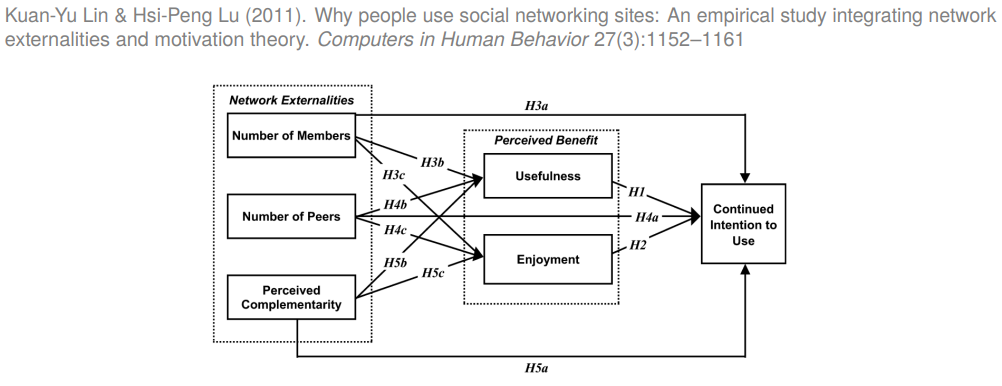
\includegraphics[width=1.3\linewidth]{Images/e3.png}
    \caption{Visual representation of hypothesis}
    \label{fig:enter-label}
\end{figure}
\pagebreak
\subsection{Research design}
\begin{figure}[h]
    \centering
    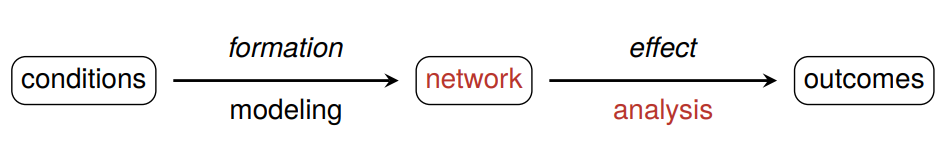
\includegraphics[width=1\linewidth]{Images/i4.png}
    \caption{networks as explanatory/intermediate/dependent variables}
    \label{fig:enter-label}
\end{figure}
\begin{figure}[h]
    \centering
    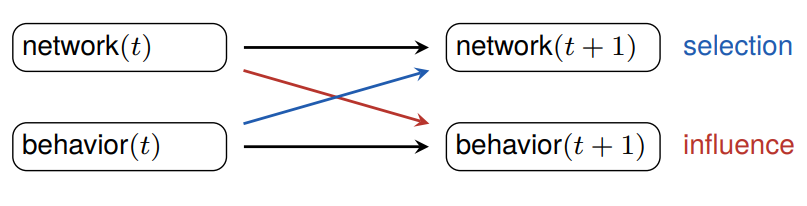
\includegraphics[width=1\linewidth]{Images/i5.png}
    \caption{Network evolution}
    \label{fig:enter-label}
\end{figure}
\subsection{Homophily as an outcome of social processes}
\begin{itemize}
    \item \textbf{social selection}: Selected people/things/pets similar to you
    \item \textbf{social influence}: Changing yourself due to you social environment
\end{itemize}
\subsection{Data}
\begin{itemize}
    \item \textbf{Data}: values of variables
    \item \textbf{Variables}: mapping from domain (units of observation) to range (potential values)
    \item $x : S\rightarrow\chi$ (x = variable; $\chi$ = range; S = domain)
\end{itemize}
\begin{figure}[h]
    \centering
    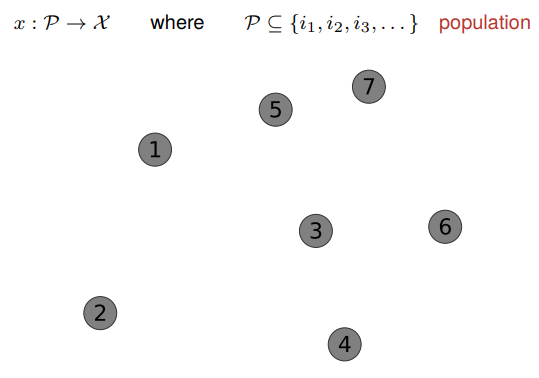
\includegraphics[width=0.7\linewidth]{Images/i6.png}
    \caption{data with unstructured domains}
    \label{fig:enter-label}
\end{figure}
\begin{figure}[h]
    \centering
    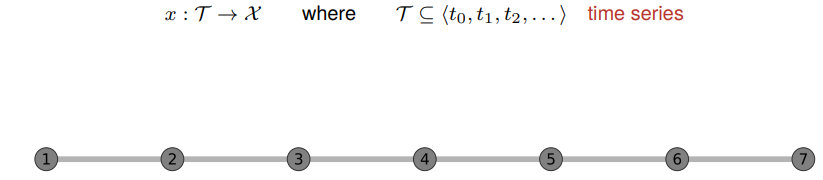
\includegraphics[width=0.7\linewidth]{Images/i7.png}
    \caption{data with structured domains}
    \label{fig:enter-label}
\end{figure}
\begin{figure}[h]
    \centering
    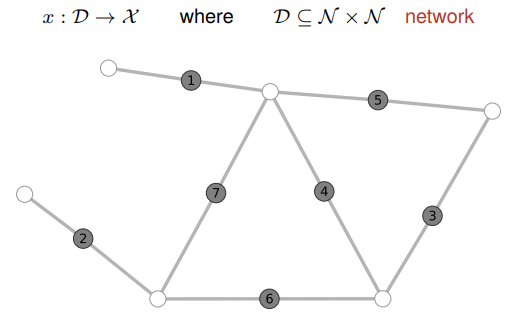
\includegraphics[width=0.7\linewidth]{Images/i8.png}
    \caption{data with structured domains}
    \label{fig:enter-label}
\end{figure}
\subsubsection{Network data}
\begin{figure}
    \centering
    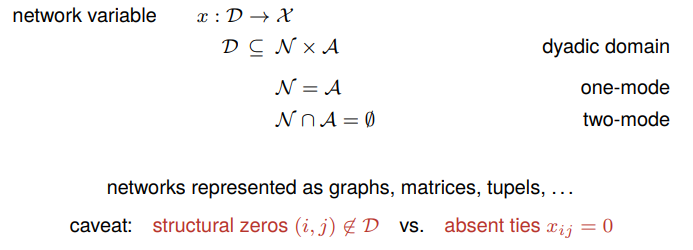
\includegraphics[width=0.7\linewidth]{Images/i9.png}
    \caption{Description of network data}
    \label{fig:enter-label}
    \textbf{Important:} Structural zeros are relations that do not need consideration (e.g. relation between yourself with yourself); we should choose values which do not influence the other important calculations for these relations (usually 0 or 1)
\end{figure}
\subsection{Types of networks}
\begin{itemize}
    \item \textbf{Two-mode network}: e.g. presence of individuals at events
    \item \textbf{one-mode network}: e.g. marriage relationships between families
\end{itemize}
\end{document}
